\subsection{Temps}
\label{section:temps}

Dans la section \ref{subsubsection:time}, nous avons pu voir qu'il est important de gérer le temps que l'application voit s'écouler. En section \ref{section:work:time}, nous avons présenté l'implémentation qui a été choisie pour résoudre cette problématique. Maintenant, nous souhaitons évaluer ses performances.

\subsubsection{Protocole}
Pour évaluer notre implémentation nous n'allons pas utiliser les mêmes expériences que pour le réseau de communications car le but ici est d'intercepter les fonctions temporelles.

L'objectif principal étant de montrer qu'il est possible de faire de la virtualisation légère, nous souhaitons mesurer le surcoût ajouté par cette interception lors de l'exécution de Simterpose. Si ce surcoût est acceptable, on pourra considérer qu'il est également possible de mettre en place une virtualisation légère qui gère cette fonctionnalité. Nos expériences vont donc consister à comparer les temps d'exécution d'une application utilisant Simterpose avec et sans interception via \texttt{LD\_PRELOAD} pour chaque type de médiation. Néanmoins, nous pensons que le changement de médiation ne devrait pas influer sur les performances car chaque médiation intervient uniquement lorsqu'on souhaite effectuer des appels systèmes réseaux que l'on fasse de l'interception avec \texttt{LD\_PRELOAD} ou pas.

L'application qui a été créée pour effectuer nos expériences exécute différents appels à des fonctions temporelles (\texttt{ftime}, \texttt{time}, \texttt{gettimeofday}, \texttt{localtime}, \texttt{mktime}...). Le protocole utilisé pour exécuter l'application est le même que celui utilisé pour tester le réseau de communications de Simterpose.

\subsubsection{Full mediation}
 Tout d'abord nous allons exécuter l'application qui effectue les appels temporels avec Simterpose en \textit{full mediation} sans \texttt{LD\_PRELOAD} et avec \texttt{LD\_PRELOAD}. Les résultats de l'expérience sont présentés Figure \ref{Temps_FM}. On constate que le temps d'exécution avec interception via \texttt{LD\_PRELOAD} est plus ou moins constant (environ 1,03 secondes), alors que celui sans interception varie énormément, entre 0,82 et 1,13 secondes. Cela est dû au fait que lorsqu'on appelle des fonctions temporelles sans interception via \texttt{LD\_PRELOAD} la bibliothèque \texttt{VDSO} est appelée pour gérer l'appel et accéde elle-même à la mémoire. Cet accès n'a pas un coût constant puisqu'il dépend de la charge du système qui varie en permanence même si on ne fait tourner que notre application et aucune autre en parallèle. Ainsi, le temps d'exécution peut varier comme c'est la cas ici alors qu'il est stable quand on utilise \texttt{LD\_PRELOAD} puisqu'on empèche ces accès. Néanmoins, en moyenne les deux expériences ont environ le même temps d'exécution, 1 seconde pour la première et 1,02 secondes pour la deuxième. On peut donc considérer que l'interception via \texttt{LD\_PRELOAD} a un surcoût négligeable lorsqu'on utilise Simterpose en \textit{full mediation}.

\begin{figure}[H]
  \centering
    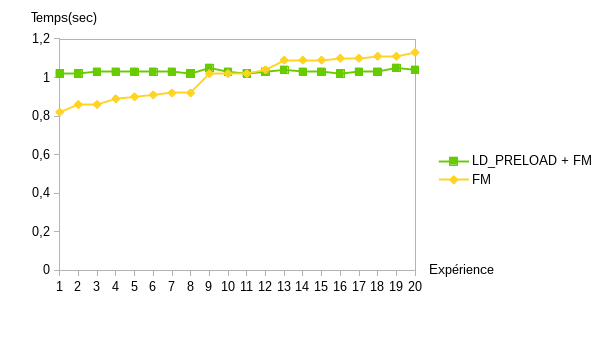
\includegraphics[scale=0.80]{mesures/graph/Temps_FM.png}
    \caption[Temps d'exécution d'une application temporelle en \textit{full mediation}] {Temps d'exécution d'une application temporelle en \textit{full mediation} avec interception via \texttt{LD\_PRELOAD} et sans interception.}
    \label{Temps_FM}
\end{figure}

\subsubsection{Address translation}
Nous allons maintenant voir s'il en est de même  lorsqu'on exécute l'application qui effectue les appels temporels avec Simterpose en \textit{address translation} avec et sans intercpetion via \texttt{LD\_PRELOAD}. Les résultats cette expérience sont présentés Figure \ref{Temps_AT}. On constate ici aussi que le temps d'exécution avec interception via \texttt{LD\_PRELOAD} est plus ou moins constant (environ 1,02 seconde), alors que celui sans interception varie beaucoup, entre 0,86 et 1,12 secondes. Cela est dû comme précédement à l'utilisation de la bibliothèque \texttt{VDSO} en l'absence d'interception via \texttt{LD\_PRELOAD}. De plus, le temps d'exécution moyen des deux expériences est le même: 1,02 secondes. Dans ce cas, on peut dire que l'interceprtion via \texttt{LD\_PRELOAD} en \textit{address translation} n'a aucun surcoût.

\begin{figure}[H]
  \centering
    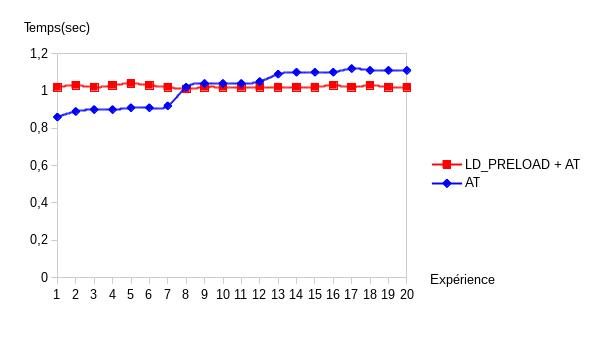
\includegraphics[scale=0.65]{mesures/graph/Temps_AT.jpg}
    \caption[Temps d'exécution d'une application temporelle en \textit{address translation}]{Temps d'exécution d'une application temporelle en \textit{address translation} avec interception via \texttt{LD\_PRELOAD} et sans interception.}
    \label{Temps_AT}
\end{figure}


Ainsi, nous avons pu voir que le surcoût dû à l'interception des fonctions temporelles via \texttt{LD\_PRELOAD} est inexistant en \textit{address translation} et qu'il est négligeable \textit{full mediation} (environ 2\%). On peut donc considérer que nous avons réussi à mettre en place une virtualisation légère qui gère également l'écoulement du temps et qui plus est de façon particulièrement efficace. De plus, en comparant les deux graphiques présentés Figure \ref{Temps_FM} et \ref{Temps_AT}, on voit bien que les courbes d'interception via \texttt{LD\_PRELOAD} se superposent et qu'il en est de même pour celles sans interception quelque soit la médiation utilisée. Le changement de médiation n'influe donc par sur les performances d'interception avec \texttt{LD\_PRELOAD}. Cela confirme l'hypothèse que nous avions fait.

\vspace{0.5cm}
